\begin{frame}{Persistent Homology in Dimension 0 (Clustering)}
\begin{center}
\begin{tikzpicture}[scale = 1]
    \draw plot[mark=*, mark size = 0.5, only marks] file {data/clust1.txt};
    \draw plot[mark=*, mark size = 0.5, only marks] file {data/clust2.txt};
\end{tikzpicture}
\begin{itemize}
\item<1-> Start with a set of data in a metric space. Set $r=0$.
\item<2-> Increase $r$. Create an edge between two points whenever the distance between them is less than $r$. This creates a graph.
\item<3-> The graph defines a simplicial complex via Vietoris-Rips.
\item<4-> If a topological property (like a Betti number) \textit{persist} over a large range of $r$, we can conclude something about the structure of the data.
\item<4-> In this case, we should expect to see $\beta_0=2$ over a large range of $r$. 
\end{itemize}
\end{center}
\end{frame}
%--------------------------------------------------------
\begin{frame}{Persistent Homology in Dimension 0 (Clustering)}
\begin{center}
\begin{tikzpicture}[scale = 1]
    \draw plot[mark=*, mark size = 0.5] file {data/clust1.txt};
    \draw plot[mark=*, mark size = 0.5] file {data/clust2.txt};
\end{tikzpicture}
\end{center}
\begin{itemize}
\item<1-> A graph similar to this should persist over a large range of $r$.
\item<2-> How could we see the clusters if these data did not lie in $\mathbb{R}^2$?
\end{itemize}
\end{frame}
%-----------------------------------------------------
\begin{frame}{RIPSER}
\begin{itemize}
\item<1-> There are several programs that do persistence.
\item<2-> We shall first look at RIPSER\cite{bauer2017ripser}.
\item<3-> Developed by Ulrich Bauer, RIPSER is a very fast C++ program for computing Vietoris-Rips persistence barcodes.
\item<4-> Let's try this on our data with two clusters.
\end{itemize}
\end{frame}
%-----------------------------------------------------
\begin{frame}{RIPSER}
\begin{center}
\begin{tikzpicture}[scale = 1]
    \draw plot[mark=*, mark size = 0.5, only marks] file {data/data1.txt};
\end{tikzpicture}
\end{center}
\begin{itemize}
\item<1-> Go to github to get the data. These data are stored as a point cloud.
\begin{center}
\hyperref[https://github.com/MatthewZabka/MAA-NCS18.git]{\textcolor{blue}{\texttt{https://github.com/MatthewZabka/MAA-NCS18.git}}}
\end{center}
\item<2-> Input \texttt{data1.txt} into RIPSER:
\begin{center}
\hyperref[https://live.ripser.org/]{\textcolor{blue}{\texttt{https://live.ripser.org/}}}
\end{center}
\end{itemize}
\end{frame}
%------------------------------------------------------
\begin{frame}{Persistent Homology}
\begin{itemize}
\item<1-> Suppose we have data that lie on the circle.
\begin{center}
\begin{figure}
\begin{tikzpicture}[scale = 1.5]
    \draw plot[mark=*, mark size = 0.5, only marks] file {data/data2.txt};
\end{tikzpicture}
\caption{An unrealistic example \texttt{data2.txt}, where data lie perfectly on $S^1$.}
\end{figure}
\end{center}
\item<2-> Input \texttt{data2.txt} into RIPSER.
\item<2-> Wait \ldots data are never this nice.
\end{itemize}
\end{frame}
%------------------------------------------------------
\begin{frame}{Persistent Homology}
\begin{itemize}
\item<1-> Suppose we have data that \textbf{almost} lie on the circle.
\begin{center}
\begin{figure}
\begin{tikzpicture}[scale = 1.5]
    \draw plot[mark=*, mark size = 0.5, only marks] file {data/data3.txt};
\end{tikzpicture}
\caption{A slightly more realistic example \texttt{data3.txt}.}
\end{figure}
\end{center}
\item<2-> Why is this also not realistic or impressive?
\end{itemize}
\end{frame}
%------------------------------------------------------
\begin{frame}{Persistent Homology}
\begin{center}
\begin{figure}
\begin{tikzpicture}[scale = 0.5]
    \draw plot[mark=*, mark size = 0.5, only marks] file {data/data3.txt};
\end{tikzpicture}
\caption{\texttt{data3.txt}.}
\end{figure}
\end{center}
\begin{itemize}
\item Now it is your turn!
\item Input \texttt{data3.txt} into RIPSER. Confirm that one generator for $H_0$ and one generator for $H_1$ persist.
\item Try inputting \texttt{data4.txt} into RIPSER up to distance 2. What can you say about the data's shape?
\item Try some real data! \texttt{data5.txt} (up to distance 150) and \texttt{data6.txt} (up to distance 2)
\item Data are located in the \texttt{data} folder that you have already downloaded!
\end{itemize}
\end{frame}
%------------------------------------------------------
\begin{frame}{Persistent Homology}
\begin{center}
{\Huge Discussion}
\end{center}
\end{frame}
%------------------------------------------------------
\begin{frame}{Combining Persistence and Other Methods}
\begin{itemize}
\item Suppose we had a barcode in dimension 1 that looked as follows:
\begin{figure}
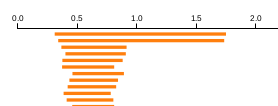
\includegraphics[scale=0.5]{images/torusbar.png}
\end{figure}
\item What are are possibilities for the manifold on which the data lie?
\end{itemize}
\end{frame}
%------------------------------------------------------
\begin{frame}{Combining Persistence and Other Methods}
\begin{itemize}
\item Suppose we had a barcode in dimension 1 that looked as follows:
\begin{figure}
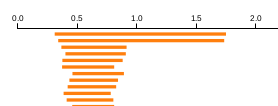
\includegraphics[scale=0.5]{images/torusbar.png}
\end{figure}
\item What are are possibilities for the manifold on which the data lie?
\end{itemize}
\end{frame}
%------------------------------------------------------
\begin{frame}{Combining Persistence and Other Methods}
\begin{itemize}
\item Suppose we had a barcode in dimension 1 that looked as follows:
\begin{figure}
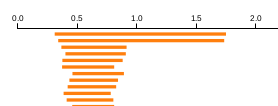
\includegraphics[scale=0.5]{images/torusbar.png}
\end{figure}
\item Suppose we perform PCA and get the following projection
\begin{figure}
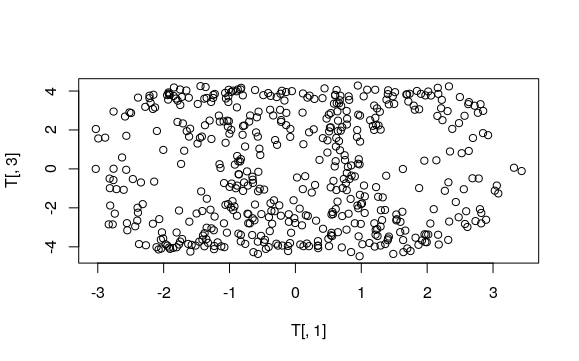
\includegraphics[scale=0.3]{images/torusPCA.png}
\end{figure}
\item What does PCA suggest about the dimension on the manifold? 
\item What does this suggest about the space on which the data lie?
\end{itemize}
\end{frame}